In order to test the robustness of LASSO, we added 5000 extra random features to the dataset in order to see if LASSO could recover the correct features. We generated the extra features by borrowing form the concept of Zipf's law. Assuming that we can calculate the frequency of a term by the percentage of times it appears as a non-zero values in the data matrix, the sorted ranking of the frequency of the terms should follow Zipf's law.  As this ranking should prove different for terms in documents in the target class compared to terms outside the target class we plotted the rank vs. frequency for the full sorted, target class [yes class], and non-target class [no class] in Figure~\ref{fig:largecompare}b. In Figure~\ref{fig:largecompare}b we present the same distributions, all however sorted by the rank of the full matrix. Non of these figure exactly depicts Zipf's law, and as such we randomly sample from this generated distribution to determine the frequency of the new randomly generated feature and randomly select either 1 or 0 for each example with probability equal to sampled frequency. In this way we generated new features which holds true the distribution of the entire feature space.



\begin{figure}[!ht]
\centering
\subfloat[L1 regularization]{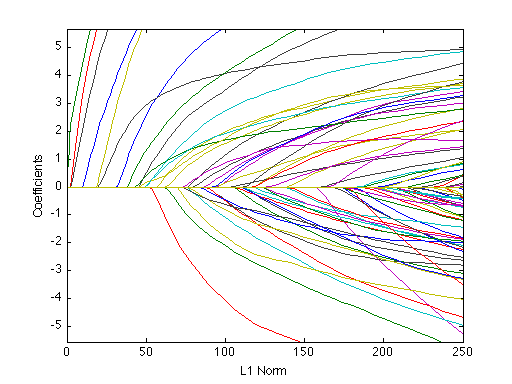
\includegraphics[width=.5\textwidth]{../images/lassoCoeffCurve.png}}
\subfloat[L2 regularization]{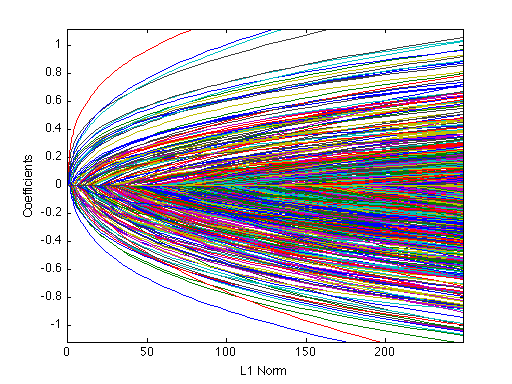
\includegraphics[width=.5\textwidth]{../images/ridgeCoeffCurve.png}}
\caption{Coefficient Paths for Regularized Logistic Regression}
%\label{fig:Coeff_paths}
\end{figure}


\begin{center}
\begin{figure}[!ht]
\centering
\subfloat[Unsorted]{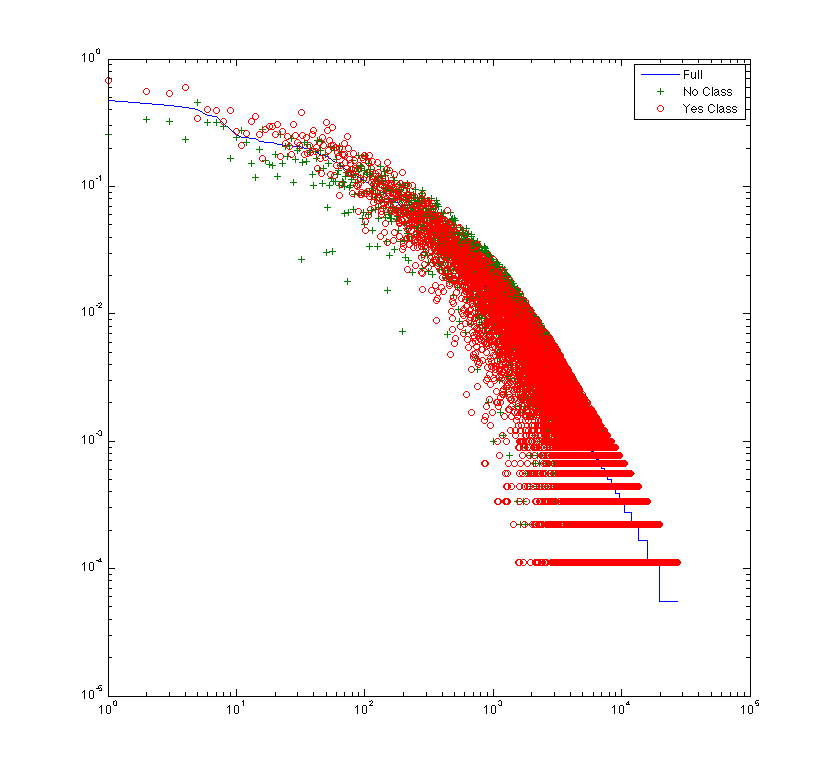
\includegraphics[width=.5\textwidth]{../images/zipfRankedFull.png}}
\subfloat[Sorted]{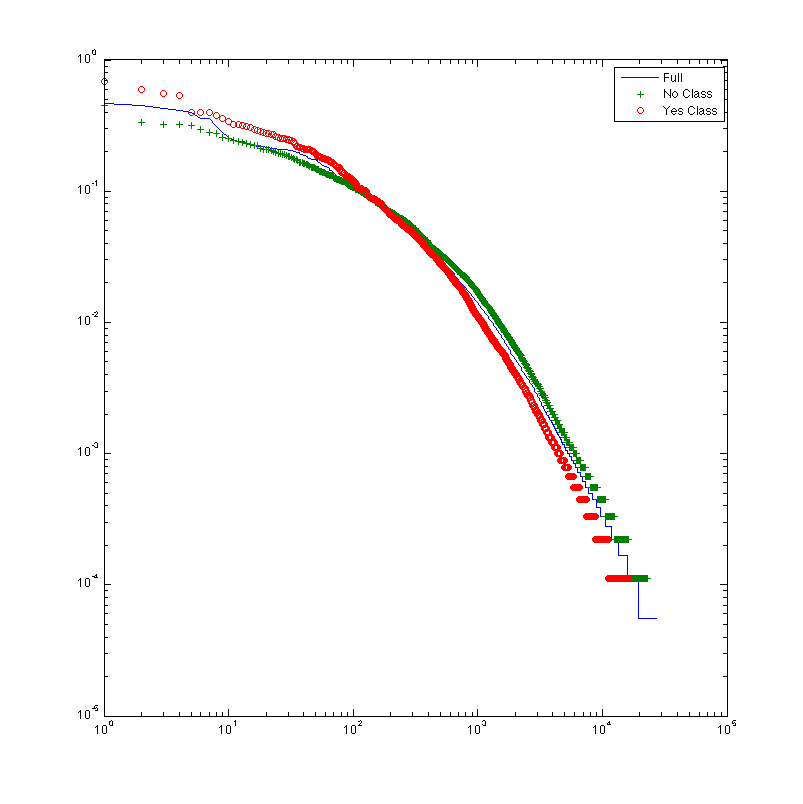
\includegraphics[width=.5\textwidth]{../images/zipfAllSorted.png}}
\caption{Frequency Vs. Rank in full data, target, and other classes}
\label{fig:largecompare}
\end{figure}
\end{center}

\begin{center}
\begin{figure}[!ht]
\centering
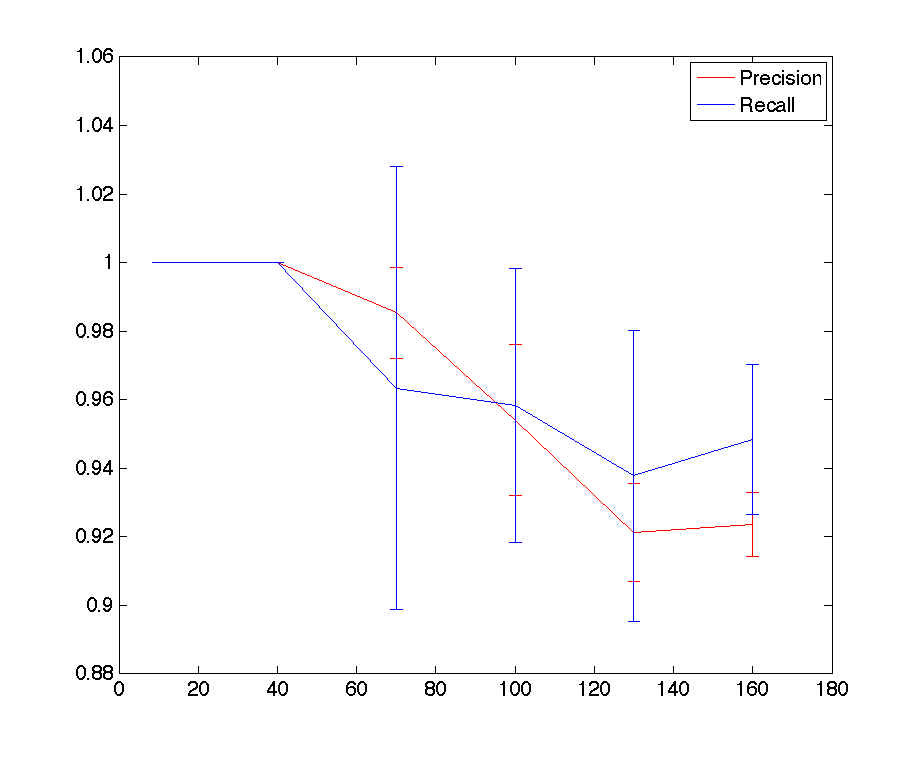
\includegraphics[width=.7\textwidth]{../images/precisionrecallExpansion.png}
\caption{Precision and Recall vs. Number of features selected using LASSO.}
\label{fig:precrecall}
\end{figure}
\end{center}

The experiment for recovering features was performed as follows. The expanded dataset was training using LASSO as well as the original dataset. The best performing lambda value was selected for both using a development set and the results compared for the training set. The accuracy of the resulting classifications were calculated as well as Precision and Recall of returning the features that LASSO returned on the actual dataset. Testing was performing using 10-fold cross validation. These results can be viewed in Table~\ref{tab:expandedResult}. As can easily be seen, LASSO has been shown to be robust for selecting good features even with the addition of random features. The mean accuracy of Expanded and Native are within the errors of each other. The calculated benefit of performing LASSO on the native dataset compared to the expanded (calculated as the average of the difference of the accuracy on each run) is none. Recall is significant at greater than 94 percent average (with large std due to one outlier), while precision is considerably lower. Sometimes LASSO using the expanded feature set would select a feature in the expanded portion of the dataset, but this did not appear to change the accuracy, though it this might make some downstream applications more difficult. The expanded dataset on average did not deviate from the native feature set (had recall and precision of 1) up until the 72 feature added with non-zero weight. This result further shows the robustness of LASSO to random feature.

These metrics were also calculated for the number of dimensions that were weighted non-zero by LASSO. These results can be viewed in Figure~\ref{fig:precrecall}. Here it can be seen up to a large number of non-zero weighted features that Precision and Recall stay at levels larger than 90 percent. The maximum number of features selected by LASSO was about 200.

\begin{table}
\begin{tabular}{lcccccc}
\hline
&Expanded&Native&Benefit&Precision&Recall&Redundant At
\\
\hline
Mean&0.9272&0.9256&-0.0016&0.7570&0.9456&72.5000 \\
STD&0.0099&0.0123&0.0069&0.2913&0.1662&9.6982
\end{tabular}
\caption{Results for expanded dataset feature selection experiment}
\label{expandedResult}
\end{table}